\chapter{Enhanced 8-point and 5-point reconstruction}\label{chap:enh_5_8_point}
As indicated in a similar research (Chapter 3), it is very attractive to use additional data to enhance reconstruction and reduce ambiguity in finding correct solution for 3D reconstruction. Previous approach of 3-point translation estimation still relayed on accuracy of camera rotation estimation. This still influences precision of final 3D reconstruction. As shown in tables \ref{fig:rot_tests_01} and \ref{fig:rot_tests_02} sensor fusion estimated rotation has few degrees error around each axis. This chapter shows how slightly noisy camera rotation angles can still be successfully used for enhancing the standard essential matrix decomposition, especially by reducing ambiguity of choosing proper $\textbf{R}$ and $\textbf{T}$.
\section{Concept - enhancing epipolar equation with initial rotation matrix} \label{sec:EpipolarEquation}
As already discussed, rotation can be distorted with noise. This can be written down as:
\begin{equation} \label{eq:Rerror}
\textbf{R} = \textbf{R}_{error}\textbf{R}_{init} 
\end{equation}
where $\textbf{R}_{init}$ is initial rotation matrix constructed from the measured angles and $\textbf{R}_{error}$ is rotation error matrix.
Looking at this from a different point of view equation \ref{eq:Rerror} one can interpret it as the multiplication of the two rotation matrices: 
one estimated initial rotation matrix (but close to local optimum - reference \ref{fig:rot_tests_01} and \ref{fig:rot_tests_02}) and the second one responsible for correction of rotation estimation noise error. 
Instead of focusing on the relative rotation matrix calculation, the primary idea of the algorithm proposed in this thesis is based on the error rotation matrix calculation. Eventually, equation \ref{eq:relativeFundamntal} can be rewritten as:
\begin{equation} \label{eq:relativeFundamntalEnhanced}
\textbf{x}_{'}^{T}\textbf{K}^{-T}\begin{bmatrix}\textbf{T}\end{bmatrix}_{x}\textbf{R}_{error}\textbf{R}_{init}\textbf{K}^{-1}\textbf{x} = 0
\end{equation}
Having notations as follows:
\begin{equation} \label{eq:leftRelative}
\begin{array}{lcl}
\textbf{p}_{'}^{T} &=& \textbf{x}_{'}^{T}\textbf{K}^{-T} \\
\textbf{p} &=& \textbf{R}_{init}\textbf{K}^{-1}\textbf{x} \\
\textbf{G} &=& \begin{bmatrix}\textbf{T}\end{bmatrix}_{x} * \textbf{R}_{error} \\
\end{array}
\end{equation}
one can notice that:
\begin{equation} \label{eq:alternativeEnhancedEquation}
\textbf{p}_{'}^{T}\textbf{G}\textbf{p} = 0
\end{equation}
which resembles the already known fundamental (Equation \ref{eq:fundamntalEquation}) and essential equations (\ref{eq:essentialEquation}). Similarly as in case of essential equation, $\textbf{p}_{'}$ and $\textbf{p}$ both are expressed in homogenous coordinates and also G has 5DOF: 2 due to an translation with unknown scale and another 3 due to an unknown error correcting angles. Such matrix problem can be resolved for instance by both 5 and 8-point algorithms (\cite{8Point}\cite{Batra5point}) and therefore used in order to retrieve both $\textbf{T}$ and $R_{error}$. \\
Calculated in such way $R_{error}$ and initial $R_{init}$ has to be multiplied in order to acquire whole camera rotation R (Equation \ref{eq:Rerror}). \\
What is more, pursuant to Appendix 6 section regarding Parametrization of 3D rotations of ''Multiple View Geometry in Computer Vision''(A6.9.1 (iii) \cite{HartleyMultipleView}), the use of Rodrigues parametrisation for small angle (and noise in initial rotation matrices estimations can be expressed by small angles) the rotation matrix can be expressed as:
\begin{equation} \label{eq:rodiguesErrorSimple}
\textbf{R}_{error} \cong \textbf{I} + \begin{bmatrix}w\end{bmatrix}_{x}
\end{equation}
and thus in our case $R_{error}$, equals approximately to:
\begin{equation} \label{eq:rodiguesError}
\textbf{R}_{error} \cong 
\begin{bmatrix*}[c]
    1   &  -w_{z}&  w_{y}\\ 
 w_{z}  &    1   & -w_{x}\\
-w_{y}  &  w_{x} &   1
\end{bmatrix*}
\end{equation} 
Such a criterion with a special matrix design can be used when decomposing \textbf{G} to $\textbf{R}_{error}$ and $\textbf{T}$ to resolve ambiguity of choosing proper rotation matrix, because only one of these two rotation matrices will fulfill this constraint. The standard four solution ambiguity with two possible rotations and translations can be reduced to two possible translation calculations. The concept described constitutes a basis of the implemented, enhanced modification in 8-point and 5-point algorithms.

\section{General algorithms modification} % top level followed by section, subsection
Most of the necessary algorithms were already implemented in OpenCV. Especially this library contains state-of-art implementation of 8-point algorithm. In addition an open-source project with the 5-point algorithm implementation was used. Its source code can be found in \cite{website:relativePoseLibrary}. \\
As could have been observed in section \ref{sec:EpipolarEquation}, in order to enhance initial pair reconstruction, the algorithms resolving the standard problems can be used, but with differently conditioned points matches (Equation \ref{eq:alternativeEnhancedEquation}). \\
The implemented enhanced 8-point and 5-point versions can be found in 'Multiview.cpp' file; their main differences are that they use sets of specially modified(conditioned) input points, which are conditioned and the first one is additionally rotated with initial rotation matrix. In OpenCV it can be done with:
\begin{lstlisting}
    ...
    undistortPoints(points1Exp, points1Exp, K, distCoeffs, rotDiffGlobal);
    undistortPoints(points2Exp, points2Exp, K, distCoeffs);
    ...
\end{lstlisting}
where rotDiffGlobal is the relative rotation matrix between two cameras. The estimated fundamental matrix needs to be transformed to essential matrix for further decomposition (Equation \ref{eq:essentialEquation}). In order to choose proper rotation and translation from SVD decomposition of calculated \textbf{G} the following code is used:
\begin{lstlisting}
void chooseProperMatrixFromEnhanced(Mat &dRx, Mat &dR1x, Mat &G, Mat &dR, Mat &T) {
    dR = dRx;
    if (decideProperMatrix(dRx, 0.05)) {
        dR = constraintMatrix(dRx);
    } else if (decideProperMatrix(dR1x, 0.05)) {
        dR = constraintMatrix(dR1x);
    } else if (decideProperMatrix(-dRx, 0.05)) {
        dR = constraintMatrix(-dRx);
    } else if (decideProperMatrix(-dR1x, 0.05)) {
        dR = constraintMatrix(-dR1x);
    }

    Mat skewT = G * dR.inv();
    cout << "skewT" << skewT << endl;

    Mat tdecx = Mat(3,1, CV_64FC1);
    tdecx.at<double>(0) = (skewT.at<double>(2,1) - skewT.at<double>(1,2))/2;
    tdecx.at<double>(1) = (skewT.at<double>(0,2) - skewT.at<double>(2,0))/2;
    tdecx.at<double>(2) = (skewT.at<double>(1,0) - skewT.at<double>(0,1))/2;
    T = tdecx;

}

bool decideProperMatrix(Mat dRot, double tolerance){
    double a00 = abs(dRot.at<double>(0,0) - 1);
    double a11 = abs(dRot.at<double>(1,1) - 1);
    double a22 = abs(dRot.at<double>(2,2) - 1);
    if((a00 + a11 + a22)/3< tolerance) {
        return true;
    }else {
        return false;
    }
}
\end{lstlisting}
These lines help to decide on a properly constrained rotation error matrix (equation \ref{eq:rodiguesError}) and calculate relative translation between cameras, but generally speaking this codes decides, which of the two error rotation matrices $\textbf{R}_error$ has all of diagonal elements equal or close to ones.
\section{Evaluation}
In the following section reader would be able to see how proposed enhancements influence camera rotation and epipolar line calculation.
\subsection{Rotation calculation tests}
In figures \ref{fig:rotation_tests_enh_01} and \ref{fig:rotation_tests_enh_02} rotation matrix decomposition to euler angles for all previous approaches along with 8-point and 5-point as well as their enhanced versions are presented. All of 8-point and 5-point versions accuracies were calculated from automatically matched correspondences, which included unfortunately as usually some outliers. \\
In blue once again reference values are marked. Most accurate estimations were presented in green and worst ones were presented in red. Enhanced version even in presence of outliers gives better estimations than standard version. In both cases 8-point enhanced version even with presence of outliers gives slightly more accurate rotation angles estimations than Sensor Fusion.
\begin{figure}[h!]
    \centering
    \includegraphics[width=0.8\textwidth]{rotation_tests_enh_01}
    \caption[Rotation tests comparison for all proposed approaches - 1st example]{Rotation tests comparison for all proposed approaches for 0.jpg and 1.jpg images. In first raw reference angles were calculated for proper point matching. Next raw shows how outliers influence those measurements. 3rd shows calculation using Sensor Fusion approach and 4th one measurements from automatic OpenCV supported matching. 5th row presents angles calculated for 8-point enhanced version. Next two rows presents 5-point algorithm both in standard and enhanced version. All angle differences are referenced to the 1st row. In green the most accurate result is presented. In red the worst one.}
    \label{fig:rotation_tests_enh_01}
\end{figure}
\begin{figure}[h!]
    \centering
    \includegraphics[width=0.8\textwidth]{rotation_tests_enh_02}
    \caption[Rotation tests comparison for all proposed approaches - 2nd example]{Rotation tests comparison for all proposed approaches for 0.jpg and 2.jpg images. In first raw reference angles were calculated for proper point matching. Next raw shows how outliers influence those measurements. 3rd shows calculation using Sensor Fusion approach and 4th one measurements from automatic OpenCV supported matching. 5th row presents angles calculated for 8-point enhanced version. Next two rows presents 5-point algorithm both in standard and enhanced version. All angle differences are referenced to the 1st row. In green the most accurate result is presented. In red the worst one.}
    \label{fig:rotation_tests_enh_02}
\end{figure}
\clearpage
\subsection{Epipolar line calculation}
In figures \ref{fig:f_01_8point_epi_comp} - \ref{fig:f_02_5point_epi_comp} epipolar lines calculation effects for both standard 8-point and 5-point algorithms as well as their enhanced versions were presented. Interesting that 8-point enhanced version slightly straightens epipolar lines in comparison to standard one. These are more similar to perfect matching cases in figures \ref{fig:f_01_epi} and \ref{fig:f_02_epi} - probably due to smaller rotation angle errors. \\
In case of 5-point algorithm for 1st tested pair (Figure \ref{fig:f_01_5point_comp}), enhanced version produced much more accurate results both in epipolar lines, probably due to more accurate euler angles calculations. There was not enough time, but it would be good to research, why in case of 5-point algorithm results are so inconsistent (one time better, other worse). \\
Evaluation of time efficiency and numerical accuracy are conducted in Chapter \ref{sec:Testin2Views}. \\
Next chapter will describe validation of authors experiments with usage of Sensor Fusion on whole Structure From Motion process.
\begin{figure}[h!]
    \centering
    \includegraphics[width=0.8\textwidth]{f_01_8point_comp}
    \caption[Comparison of epipolar lines for 8-point standard and enhanced versions  - 1st example]{Comparison of epipolar lines for 8-point standard (upper) and enhanced versions (bottom) for automatically matched points in images 0.jpg and 1.jpg from test dataset. Some outliers are produced during feature matching process.}
    \label{fig:f_01_8point_epi_comp}
\end{figure}

\begin{figure}[h!]
    \centering
    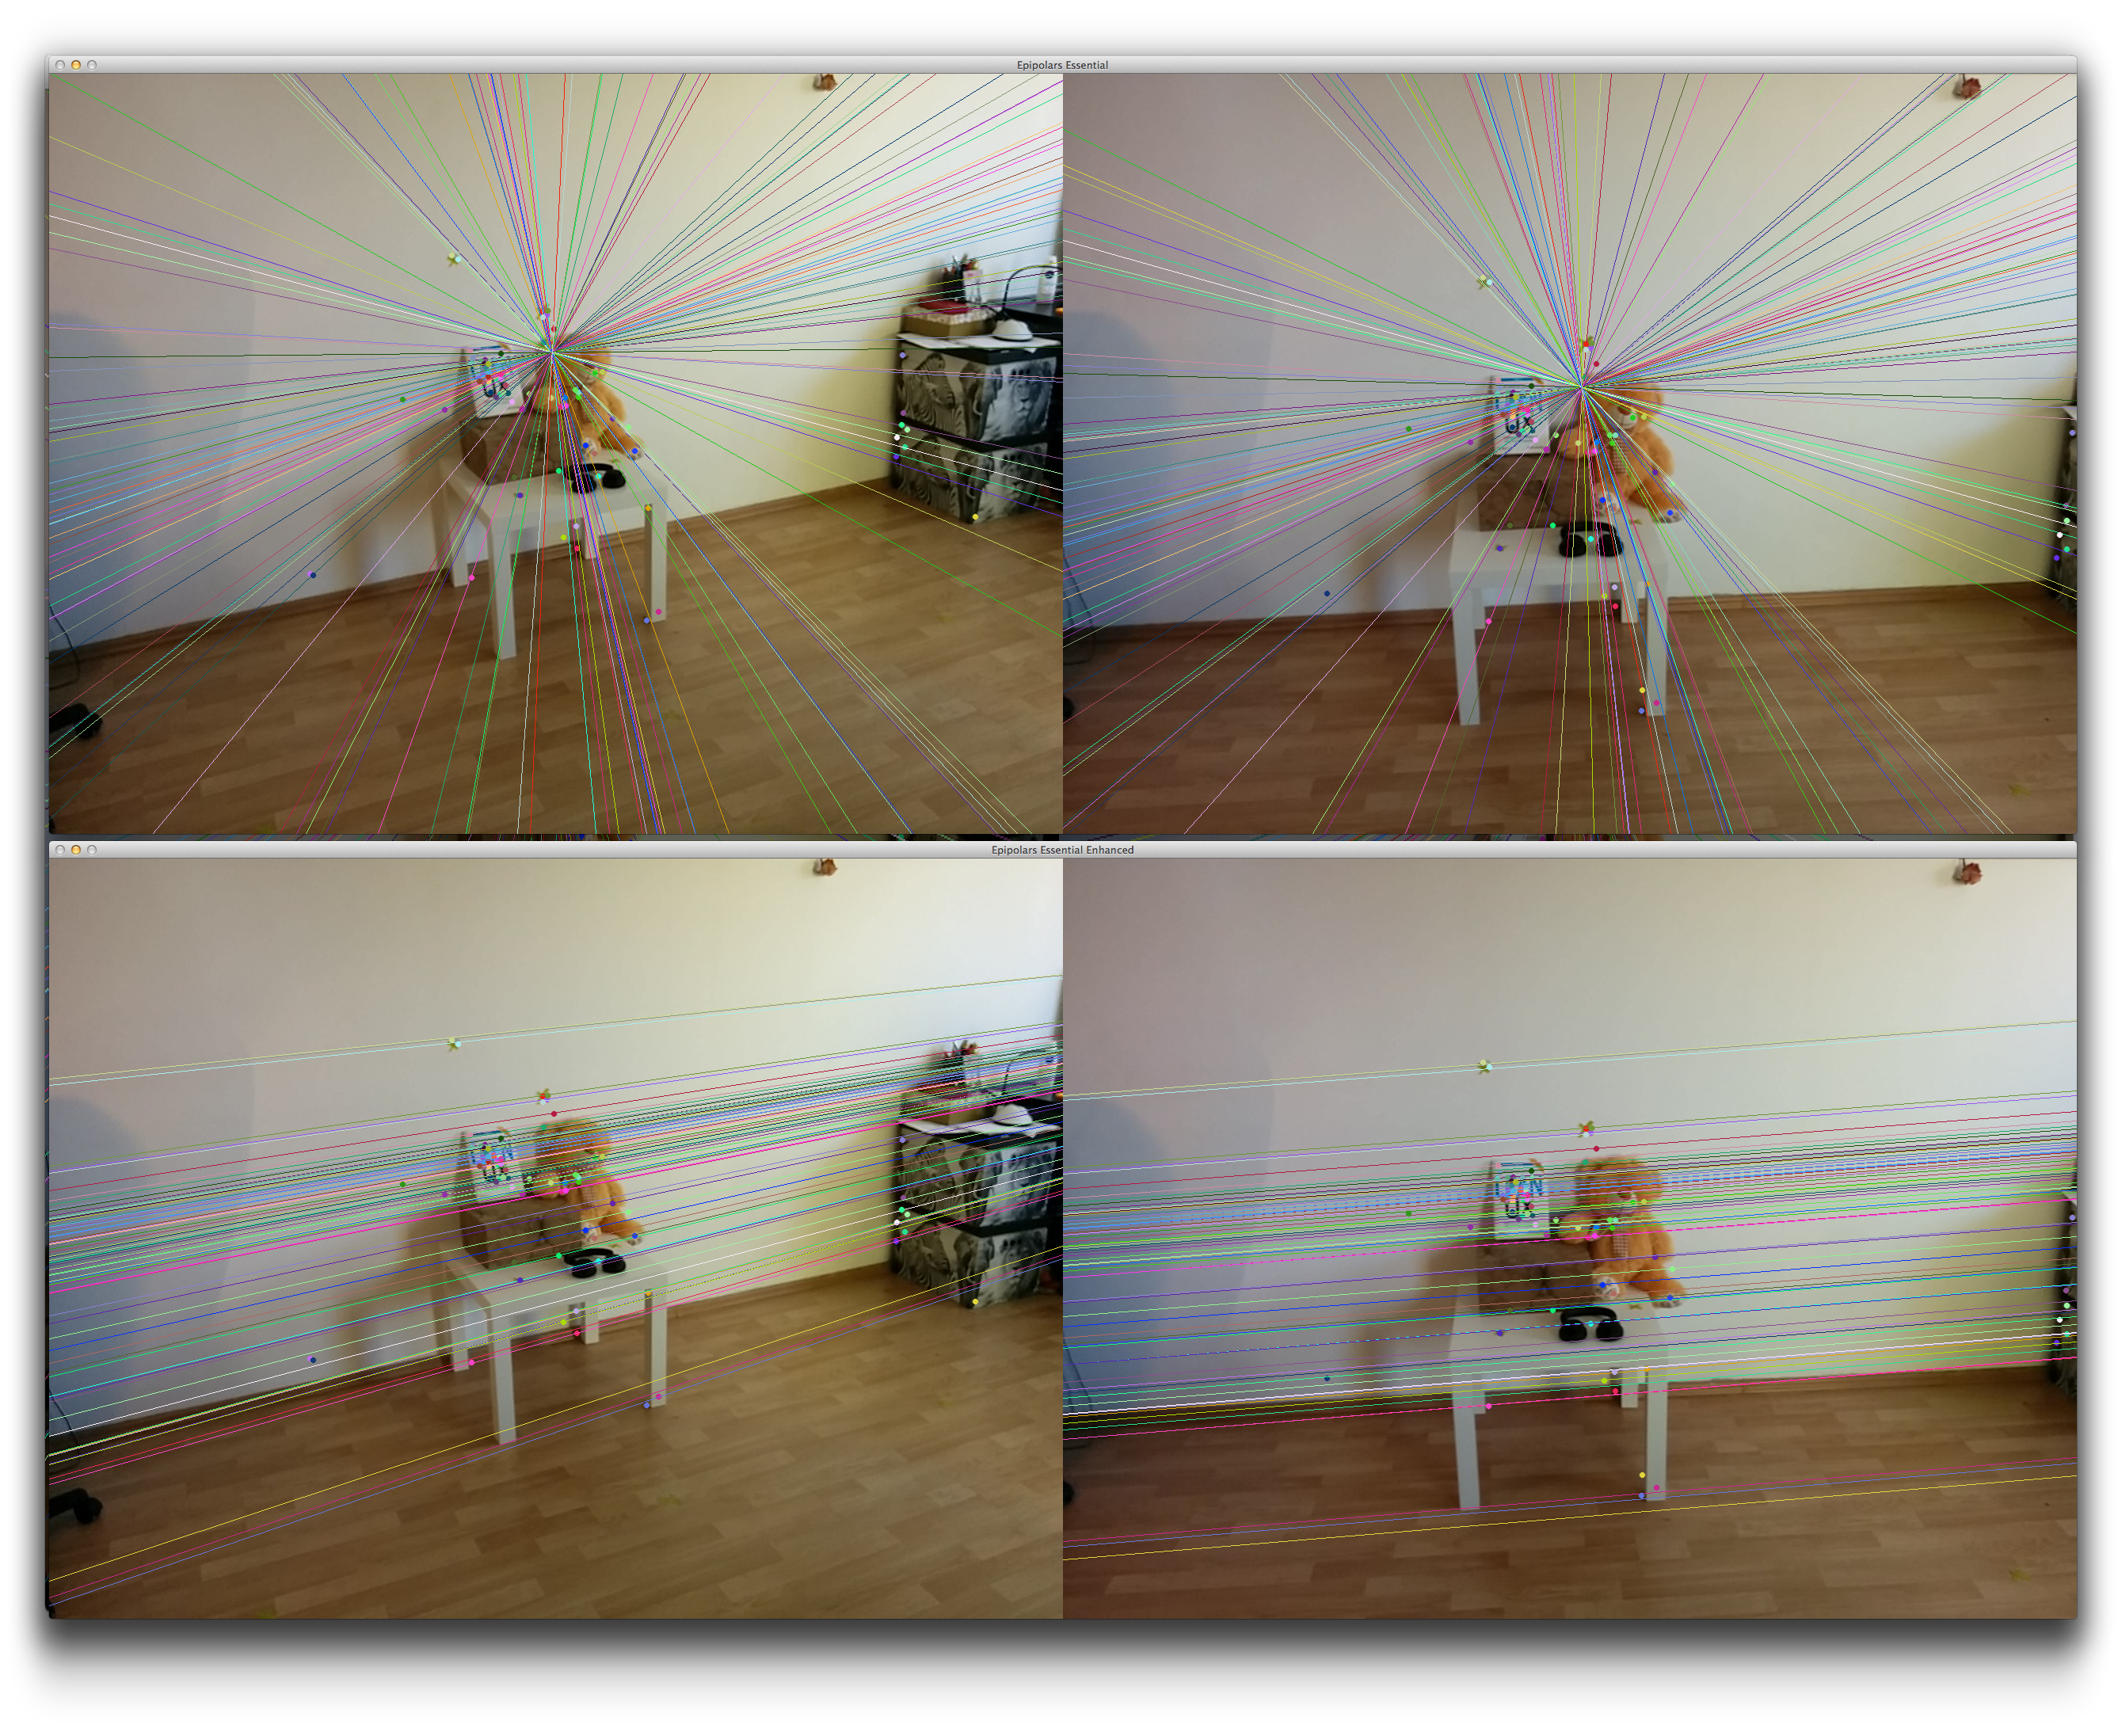
\includegraphics[width=0.8\textwidth]{f_01_5point_comp}
    \caption[Comparison of epipolar lines for 5-point standard and enhanced versions  - 1st example]{Comparison of epipolar lines for 5-point standard (upper) and enhanced versions (bottom) for automatically matched points in images 0.jpg and 1.jpg from test dataset. Some outliers are produced during feature matching process.}
    \label{fig:f_01_5point_comp}
\end{figure}

\begin{figure}[h!]
    \centering
    \includegraphics[width=0.8\textwidth]{f_02_8point_comp}
    \caption[Comparison of epipolar lines for 8-point standard and enhanced versions  - 2nd example]{Comparison of epipolar lines for 8-point standard (upper) and enhanced versions (bottom) for automatically matched points in images 0.jpg and 2.jpg from test dataset. Some outliers are produced during feature matching process.}
    \label{fig:f_02_8point_epi_comp}
\end{figure}

\begin{figure}[h!]
    \centering
    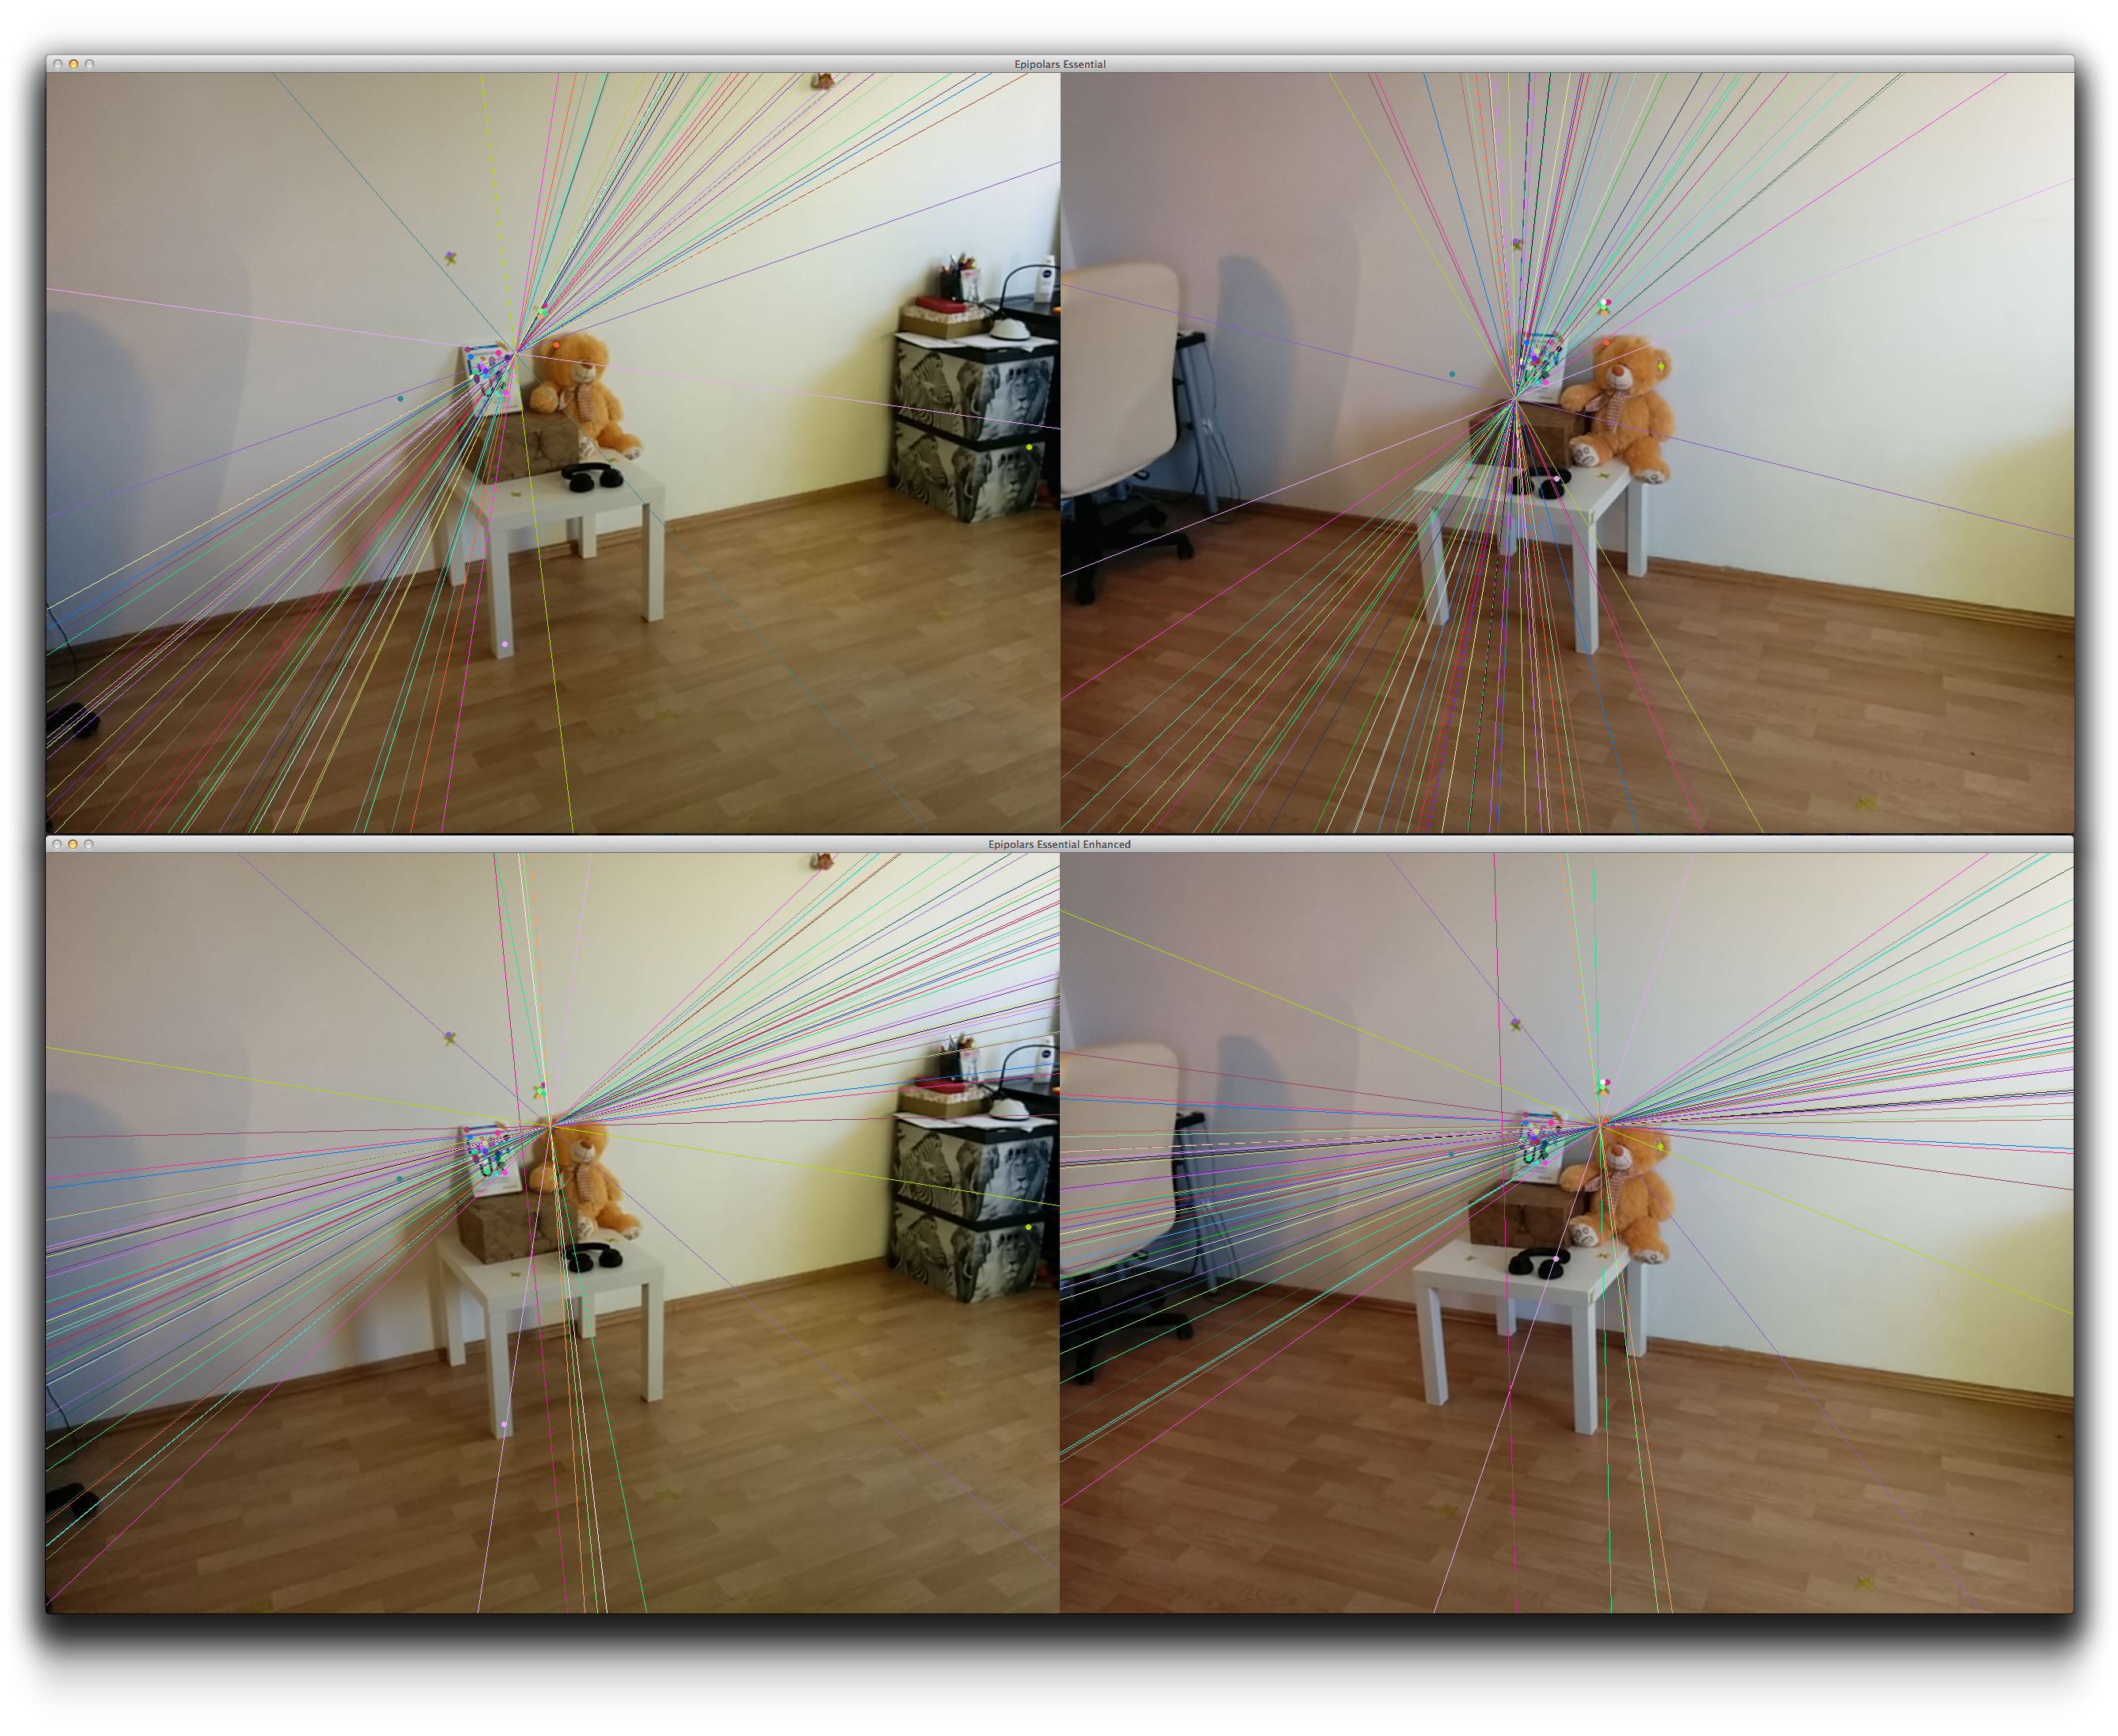
\includegraphics[width=0.8\textwidth]{f_02_5point_comp}
    \caption[Comparison of epipolar lines for 5-point standard and enhanced versions  - 2nd example]{Comparison of epipolar lines for 5-point standard (upper) and enhanced versions (bottom) for automatically matched points in images 0.jpg and 2.jpg from test dataset. Some outliers are produced during feature matching process.}
    \label{fig:f_02_5point_epi_comp}
\end{figure}


